\section{未命名节}

\subsection{循环神经网络的梯度分析}

\subsection{8.7.1 循环神经网络的梯度分析}

\subsection{8.7.1 循环神经网络的梯度分析}
\begin{center}
\Large \textcolor{blue}{RNN的梯度是如何计算的?}
\end{center}


\paragraph{回顾:RNN的前向传播}
\textbf{RNN的核心公式:}
\begin{align*}
\mathbf{h}_t &= \tanh(\mathbf{W}_{xh}\mathbf{x}_t + \mathbf{W}_{hh}\mathbf{h}_{t-1} + \mathbf{b}_h) \\
\mathbf{o}_t &= \mathbf{W}_{hq}\mathbf{h}_t + \mathbf{b}_q \\
\mathcal{L}_t &= \ell(\mathbf{o}_t, y_t)
\end{align*}

\textbf{总损失:}
$$\mathcal{L} = \frac{1}{T}\sum_{t=1}^{T}\mathcal{L}_t$$

\begin{center}
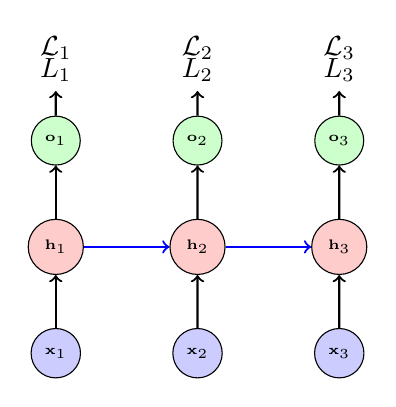
\begin{tikzpicture}[scale=0.9]
% 时间步
\foreach \t in {1,2,3} {
    \node[circle,draw,fill=red!20,minimum size=0.7cm] (h\t) at (\t*2,1.5) {\tiny$\mathbf{h}_{\t}$};
    \node[circle,draw,fill=blue!20,minimum size=0.6cm] (x\t) at (\t*2,0) {\tiny$\mathbf{x}_{\t}$};
    \node[circle,draw,fill=green!20,minimum size=0.6cm] (o\t) at (\t*2,3) {\tiny$\mathbf{o}_{\t}$};
    \node[above] (l\t) at (\t*2,3.7) {$L_{\t}$};
    
    \draw[->,thick] (x\t) -- (h\t);
    \draw[->,thick] (h\t) -- (o\t);
    \draw[->,thick] (o\t) -- (l\t);
}

\draw[->,thick,blue] (h1) -- (h2);
\draw[->,thick,blue] (h2) -- (h3);

\node[above] at (2,4) {$\mathcal{L}_1$};
\node[above] at (4,4) {$\mathcal{L}_2$};
\node[above] at (6,4) {$\mathcal{L}_3$};

\end{tikzpicture}
\end{center}


\paragraph{BPTT的核心思想}
\textbf{通过时间反向传播(Backpropagation Through Time)}

\begin{center}
\begin{tikzpicture}[scale=0.9]
% 前向传播
\node[above] at (2,3.5) {\small 前向传播};
\foreach \t in {1,2,3,4} {
    \node[circle,draw,fill=blue!20,minimum size=0.8cm] (h\t) at (\t*1.8,2) {\tiny$\mathbf{h}_{\t}$};
}
\draw[->,thick,red] (h1) -- (h2);
\draw[->,thick,red] (h2) -- (h3);
\draw[->,thick,red] (h3) -- (h4);
\node[right] at (7.5,2) {$\rightarrow$ 时间};

% 反向传播
\node[above] at (2,0.5) {\small 反向传播};
\foreach \t in {1,2,3,4} {
    \node[circle,draw,fill=red!20,minimum size=0.8cm] (b\t) at (\t*1.8,-1.5) {\tiny$\frac{\partial\mathcal{L}}{\partial\mathbf{h}_{\t}}$};
}
\draw[<-,thick,blue] (b1) -- (b2);
\draw[<-,thick,blue] (b2) -- (b3);
\draw[<-,thick,blue] (b3) -- (b4);
\node[right] at (7.5,-1.5) {$\leftarrow$ 时间};

% 说明
\node[below,text width=8cm,align=center] at (3,-2.5) {
\small 梯度\textbf{逆着}时间传播,从 $t=T$ 到 $t=1$
};

\end{tikzpicture}
\end{center}

\begin{theorem}[关键]
BPTT就是在展开的RNN计算图上应用标准的反向传播
\end{theorem}


\paragraph{计算 $\mathbf{W}
\textbf{目标:}计算 $\frac{\partial\mathcal{L}}{\partial\mathbf{W}_{hq}}$

\textbf{分析:}
$$\mathcal{L} = \frac{1}{T}\sum_{t=1}^{T}\mathcal{L}_t = \frac{1}{T}\sum_{t=1}^{T}\ell(\mathbf{o}_t, y_t)$$

由于 $\mathbf{o}_t = \mathbf{W}_{hq}\mathbf{h}_t + \mathbf{b}_q$

\begin{definition}[链式法则]
\begin{align*}
\frac{\partial\mathcal{L}}{\partial\mathbf{W}_{hq}} &= \frac{1}{T}\sum_{t=1}^{T}\frac{\partial\mathcal{L}_t}{\partial\mathbf{W}_{hq}} \\
&= \frac{1}{T}\sum_{t=1}^{T}\frac{\partial\mathcal{L}_t}{\partial\mathbf{o}_t}\frac{\partial\mathbf{o}_t}{\partial\mathbf{W}_{hq}} \\
&= \frac{1}{T}\sum_{t=1}^{T}\frac{\partial\mathcal{L}_t}{\partial\mathbf{o}_t}\mathbf{h}_t^{\top}
\end{align*}
\end{definition}

\begin{theorem}[观察]
$\mathbf{W}_{hq}$ 的梯度是各时间步梯度的\textbf{平均}
\end{theorem}


\paragraph{计算 $\mathbf{W}
\textbf{目标:}计算 $\frac{\partial\mathcal{L}}{\partial\mathbf{W}_{hh}}$

\textbf{挑战:}$\mathbf{W}_{hh}$ 在\textbf{每个时间步}都被使用

\begin{center}
\begin{tikzpicture}[scale=0.9]
% 时间步
\foreach \t in {1,2,3,4} {
    \node[circle,draw,fill=blue!20,minimum size=0.7cm] (h\t) at (\t*1.8,2) {\tiny$\mathbf{h}_{\t}$};
    \node[circle,draw,fill=red!20,minimum size=0.6cm] (l\t) at (\t*1.8,3.2) {\tiny$\mathcal{L}_{\t}$};
    \draw[->,thick] (h\t) -- (l\t);
}

% W_hh的使用
\draw[->,thick,blue] (h1) -- (h2) node[midway,above,font=\tiny] {$\mathbf{W}_{hh}$};
\draw[->,thick,blue] (h2) -- (h3) node[midway,above,font=\tiny] {$\mathbf{W}_{hh}$};
\draw[->,thick,blue] (h3) -- (h4) node[midway,above,font=\tiny] {$\mathbf{W}_{hh}$};

% 标注
\node[below,text width=8cm,align=center] at (4,0.8) {
\small $\mathbf{W}_{hh}$ 影响了\textbf{所有后续时间步}的损失
};

\end{tikzpicture}
\end{center}

\begin{definition}[关键观察]
$\mathbf{W}_{hh}$ 在时间步 $t$ 的修改会影响 $t+1, t+2, \ldots, T$ 的所有输出
\end{definition}


\paragraph{$\mathbf{W}
\textbf{链式法则:}
$$\frac{\partial\mathcal{L}}{\partial\mathbf{W}_{hh}} = \sum_{t=1}^{T}\frac{\partial\mathcal{L}}{\partial\mathbf{h}_t}\frac{\partial\mathbf{h}_t}{\partial\mathbf{W}_{hh}}$$

\textbf{问题:}$\mathbf{h}_t$ 依赖于 $\mathbf{h}_{t-1}$,而 $\mathbf{h}_{t-1}$ 也依赖于 $\mathbf{W}_{hh}$!

\begin{definition}[完整的链式法则]
对于时间步 $t$:
\begin{align*}
\frac{\partial\mathcal{L}}{\partial\mathbf{W}_{hh}} &= \sum_{t=1}^{T}\sum_{k=1}^{t}\frac{\partial\mathcal{L}}{\partial\mathbf{h}_t}\frac{\partial\mathbf{h}_t}{\partial\mathbf{h}_k}\frac{\partial\mathbf{h}_k}{\partial\mathbf{W}_{hh}}
\end{align*}
\end{definition}

\begin{theorem}[关键项]
$\frac{\partial\mathbf{h}_t}{\partial\mathbf{h}_k}$:隐状态 $\mathbf{h}_t$ 对之前隐状态 $\mathbf{h}_k$ 的梯度\\
这是梯度消失/爆炸的根源!
\end{theorem}


\paragraph{隐状态对隐状态的梯度}
\textbf{递推关系:}
$$\mathbf{h}_t = \tanh(\mathbf{W}_{hh}\mathbf{h}_{t-1} + \mathbf{W}_{xh}\mathbf{x}_t + \mathbf{b}_h)$$

\textbf{对 $\mathbf{h}_{t-1}$ 求偏导:}
$$\frac{\partial\mathbf{h}_t}{\partial\mathbf{h}_{t-1}} = \text{diag}(1-\tanh^2(\cdot))\mathbf{W}_{hh}$$

\textbf{连乘形式($t > k$):}
$$\frac{\partial\mathbf{h}_t}{\partial\mathbf{h}_k} = \prod_{i=k+1}^{t}\frac{\partial\mathbf{h}_i}{\partial\mathbf{h}_{i-1}} = \prod_{i=k+1}^{t}\text{diag}(1-\tanh^2(\cdot))\mathbf{W}_{hh}$$

\begin{theorem}[这就是问题所在!]
梯度是\textbf{多个矩阵的连乘},可能指数级增长或衰减
\end{theorem}


\paragraph{梯度消失的数学分析}
\textbf{简化分析(标量情况):}

假设 $h_t = \tanh(w \cdot h_{t-1})$

$$\frac{\partial h_t}{\partial h_k} = \prod_{i=k+1}^{t}w \cdot (1-\tanh^2(w \cdot h_{i-1}))$$

\begin{center}
\begin{tikzpicture}[scale=1.0]
% 坐标轴
\draw[->,thick] (0,0) -- (6,0) node[right] {时间步差 $t-k$};
\draw[->,thick] (0,0) -- (0,3.5) node[above] {梯度值};

% 梯度消失
\draw[blue,thick,domain=0:5,samples=50] plot (\x,{3*exp(-0.5*\x)});
\node[blue,above] at (2,2) {$|w| < 1$};
\node[blue] at (4,0.5) {梯度消失};

% 梯度爆炸
\draw[red,thick,domain=0:2,samples=50] plot (\x,{0.5*exp(0.8*\x)});
\node[red] at (1.5,2.5) {$|w| > 1$};
\node[red] at (1,3) {梯度爆炸};

\end{tikzpicture}
\end{center}

\begin{definition}[关键因素]
\begin{itemize}
    \item $|w| < 1$:梯度指数衰减 $\rightarrow$ 梯度消失
    \item $|w| > 1$:梯度指数增长 $\rightarrow$ 梯度爆炸
    \item $1-\tanh^2(\cdot) \in (0,1]$:进一步加剧消失
\end{itemize}
\end{definition}


\paragraph{为什么 $\tanh$ 导致梯度消失?}
\textbf{$\tanh$ 函数的导数:}
$$\frac{d}{dx}\tanh(x) = 1 - \tanh^2(x)$$

\begin{center}
\begin{tikzpicture}[scale=1.0]
% 坐标轴
\draw[->,thick] (-3,0) -- (3,0) node[right] {$x$};
\draw[->,thick] (0,-0.5) -- (0,2) node[above] {$y$};

% tanh曲线
\draw[blue,thick,domain=-2.5:2.5,samples=100] plot (\x,{0.9*tanh(\x)+1});
\node[blue,right] at (2,1.7) {$\tanh(x)$};

% 导数曲线
\draw[red,thick,domain=-2.5:2.5,samples=100] plot (\x,{0.9*(1-tanh(\x)^2)});
\node[red,right] at (1.5,0.5) {$1-\tanh^2(x)$};

% 标注
\draw[dashed] (-3,1) -- (3,1);
\node[left,font=\tiny] at (0,1) {1};

% 饱和区
\fill[green!20,opacity=0.3] (-3,-0.5) rectangle (-1,2);
\fill[green!20,opacity=0.3] (1,-0.5) rectangle (3,2);
\node[green!60!black,font=\tiny] at (-2,1.7) {饱和区};
\node[green!60!black,font=\tiny] at (2,0.3) {饱和区};

\end{tikzpicture}
\end{center}

\begin{theorem}[关键]
当 $|x|$ 较大时,$\tanh(x)$ 饱和,导数趋近于0 $\Rightarrow$ 梯度消失
\end{theorem}


\paragraph{梯度爆炸的例子}
\textbf{考虑矩阵的谱半径(最大特征值):}

设 $\lambda_{\max}$ 是 $\mathbf{W}_{hh}$ 的最大特征值

$$\left\|\frac{\partial\mathbf{h}_t}{\partial\mathbf{h}_k}\right\| \lesssim \lambda_{\max}^{t-k}$$

\begin{center}
\begin{tikzpicture}[scale=0.9]
% 情况1
\node[draw,fill=green!20,text width=4cm] at (0,2.5) {
$\lambda_{\max} < 1$\\
\small 梯度指数衰减\\
\footnotesize 远距离依赖学不到
};

% 情况2
\node[draw,fill=yellow!20,text width=4cm] at (0,0.8) {
$\lambda_{\max} \approx 1$\\
\small 理想情况\\
\footnotesize 梯度稳定传播
};

% 情况3
\node[draw,fill=red!20,text width=4cm] at (6,2.5) {
$\lambda_{\max} > 1$\\
\small 梯度指数增长\\
\footnotesize 训练不稳定、NaN
};

% 箭头
\draw[->,thick] (2.2,2.5) -- (3.8,2.5);
\node[above,font=\tiny] at (3,2.7) {难以控制};

\end{tikzpicture}
\end{center}

\begin{theorem}[困境]
很难找到 $\lambda_{\max} \approx 1$ 的 $\mathbf{W}_{hh}$,训练中容易漂移
\end{theorem}


\paragraph{梯度问题的可视化}
\begin{center}
\begin{tikzpicture}[scale=0.9]
% 时间步
\foreach \t in {1,2,3,4,5} {
    \node[circle,draw,fill=blue!20,minimum size=0.7cm] (h\t) at (\t*1.5,2) {\tiny$h_{\t}$};
}

% 前向传播(正常)
\draw[->,thick,blue] (h1) -- (h2);
\draw[->,thick,blue] (h2) -- (h3);
\draw[->,thick,blue] (h3) -- (h4);
\draw[->,thick,blue] (h4) -- (h5);

% 反向梯度(消失)
\draw[<-,ultra thick,red] (h1) -- (h2) node[midway,below,font=\tiny] {$\times 0.5$};
\draw[<-,ultra thick,red] (h2) -- (h3) node[midway,below,font=\tiny] {$\times 0.5$};
\draw[<-,ultra thick,red] (h3) -- (h4) node[midway,below,font=\tiny] {$\times 0.5$};
\draw[<-,ultra thick,red] (h4) -- (h5) node[midway,below,font=\tiny] {$\times 0.5$};

% 标注
\node[below] at (h1) {梯度 $\approx 0.06$};
\node[below] at (h3) {梯度 $\approx 0.25$};
\node[below] at (h5) {梯度 $= 1$};

\node[below,text width=8cm,align=center] at (4,0.3) {
\small 梯度在长序列上\textbf{指数衰减}:$1 \times 0.5^4 = 0.0625$
};

\end{tikzpicture}
\end{center}



\subsection{通过时间反向传播的细节}

\subsection{8.7.2 通过时间反向传播的细节}

\subsection{8.7.2 通过时间反向传播的细节}
\begin{center}
\Large \textcolor{blue}{BPTT的实际计算}
\end{center}


\paragraph{完整的BPTT算法}
\textbf{给定:}序列 $\mathbf{x}_1, \ldots, \mathbf{x}_T$,目标 $y_1, \ldots, y_T$

\begin{definition}[前向传播]
\textbf{for} $t = 1$ to $T$ \textbf{do}
\begin{align*}
\mathbf{h}_t &= \tanh(\mathbf{W}_{xh}\mathbf{x}_t + \mathbf{W}_{hh}\mathbf{h}_{t-1} + \mathbf{b}_h) \\
\mathbf{o}_t &= \mathbf{W}_{hq}\mathbf{h}_t + \mathbf{b}_q \\
\mathcal{L}_t &= \ell(\mathbf{o}_t, y_t)
\end{align*}
\textbf{end for}

计算总损失:$\mathcal{L} = \frac{1}{T}\sum_{t=1}^{T}\mathcal{L}_t$
\end{definition}


\paragraph{完整的BPTT算法(续)}
\begin{definition}[反向传播]
初始化:$\frac{\partial\mathcal{L}}{\partial\mathbf{h}_T} = \frac{\partial\mathcal{L}_T}{\partial\mathbf{h}_T}$

\textbf{for} $t = T$ down to $1$ \textbf{do}
\begin{align*}
\frac{\partial\mathcal{L}}{\partial\mathbf{o}_t} &= \frac{\partial\ell(\mathbf{o}_t, y_t)}{\partial\mathbf{o}_t} \\
\frac{\partial\mathcal{L}}{\partial\mathbf{h}_t} &= \frac{\partial\mathcal{L}}{\partial\mathbf{o}_t}\frac{\partial\mathbf{o}_t}{\partial\mathbf{h}_t} + \frac{\partial\mathcal{L}}{\partial\mathbf{h}_{t+1}}\frac{\partial\mathbf{h}_{t+1}}{\partial\mathbf{h}_t} \\
\frac{\partial\mathcal{L}}{\partial\mathbf{W}_{hh}} &\mathrel{+}= \frac{\partial\mathcal{L}}{\partial\mathbf{h}_t}\frac{\partial\mathbf{h}_t}{\partial\mathbf{W}_{hh}}
\end{align*}
\textbf{end for}
\end{definition}

\begin{theorem}[关键]
梯度\textbf{逐时间步累积},从 $t=T$ 反向到 $t=1$
\end{theorem}


\paragraph{BPTT的计算图}
\begin{center}
\begin{tikzpicture}[scale=0.85]
% 前向传播
\node[above] at (3,4) {\textbf{前向传播}};
\foreach \t in {1,2,3,4} {
    \node[circle,draw,fill=blue!20,minimum size=0.7cm] (h\t) at (\t*1.5,3) {\tiny$\mathbf{h}_{\t}$};
    \node[circle,draw,fill=green!20,minimum size=0.6cm] (o\t) at (\t*1.5,2) {\tiny$\mathbf{o}_{\t}$};
    \node[circle,draw,fill=orange!20,minimum size=0.6cm] (l\t) at (\t*1.5,1) {\tiny$\mathcal{L}_{\t}$};
    
    \draw[->,thick] (h\t) -- (o\t);
    \draw[->,thick] (o\t) -- (l\t);
}
\draw[->,thick,blue] (h1) -- (h2);
\draw[->,thick,blue] (h2) -- (h3);
\draw[->,thick,blue] (h3) -- (h4);

% 反向传播
\node[above] at (3,-1) {\textbf{反向传播}};
\foreach \t in {1,2,3,4} {
    \node[circle,draw,fill=red!20,minimum size=0.9cm,font=\tiny] (g\t) at (\t*1.5,-2) {$\frac{\partial\mathcal{L}}{\partial\mathbf{h}_{\t}}$};
}
\draw[<-,thick,red] (g1) -- (g2) node[midway,above,font=\tiny] {累积};
\draw[<-,thick,red] (g2) -- (g3) node[midway,above,font=\tiny] {累积};
\draw[<-,thick,red] (g3) -- (g4) node[midway,above,font=\tiny] {累积};

% 连接
\foreach \t in {1,2,3,4} {
    \draw[->,thick,dotted] (l\t) -- (g\t);
}

\end{tikzpicture}
\end{center}


\paragraph{伪代码实现}
\begin{lstlisting}[language=Python,basicstyle=\ttfamily\tiny]
def bptt(X, Y, model):
    """ BPTT X: sequence (T, batch, input_size) Y: sequence (T, batch) """
    T = X.shape[0]
    
    hiddens = []
    outputs = []
    h = torch.zeros(batch_size, hidden_size)
    
    for t in range(T):
        h = torch.tanh(X[t] @ W_xh + h @ W_hh + b_h)
        o = h @ W_hq + b_q
        hiddens.append(h)
        outputs.append(o)
    
    # loss
    loss = sum(cross_entropy(outputs[t], Y[t]) for t in range(T)) / T
    
    dh_next = torch.zeros_like(h)  # commenttime step的梯度
    
    for t in reversed(range(T)):  # commentT到1
        # Output
        do = grad_output(outputs[t], Y[t])
        
        #  = loss + futuretime step
        dh = do @ W_hq.T + dh_next
        
        # tanh
        dh_raw = dh * (1 - hiddens[t]**2)
        
        # parameters
        W_xh.grad += X[t].T @ dh_raw
        W_hh.grad += hiddens[t-1].T @ dh_raw if t > 0 else 0
        W_hq.grad += hiddens[t].T @ do
        
        # time step
        dh_next = dh_raw @ W_hh.T
    
    return loss
\end{lstlisting}


\paragraph{BPTT的内存问题}
\textbf{问题:}需要存储所有时间步的隐状态

\begin{center}
\begin{tikzpicture}[scale=0.9]
% 内存占用
\node[draw,fill=yellow!20,text width=10cm] at (5,3.5) {
\textbf{前向传播:}\\
存储 $\mathbf{h}_1, \mathbf{h}_2, \ldots, \mathbf{h}_T$\\
内存:$O(T \times H)$,$T$ 是序列长度,$H$ 是隐藏单元数
};

\draw[->,thick] (5,3) -- (5,2.6);

\node[draw,fill=red!20,text width=10cm] at (5,2.2) {
\textbf{反向传播:}\\
需要访问所有存储的隐状态\\
才能计算梯度
};

\draw[->,thick] (5,1.8) -- (5,1.4);

\node[draw,fill=orange!20,text width=10cm] at (5,1) {
\textbf{问题:}\\
$T$ 很大时(如 $T=1000$),内存爆炸!\\
例如:$T=1000, H=512, \text{batch}=32$ \\
$\Rightarrow$ $1000 \times 512 \times 32 \times 4\text{bytes} \approx 65\text{MB}$
};

\end{tikzpicture}
\end{center}


\paragraph{截断BPTT(Truncated BPTT)}
\textbf{解决方案:}只在有限时间步内反向传播

\begin{center}
\begin{tikzpicture}[scale=0.85]
% 完整序列
\node[above] at (4,3.5) {\small 完整序列(长度=12)};
\foreach \t in {1,...,12} {
    \node[circle,draw,fill=blue!20,minimum size=0.5cm,font=\tiny] (h\t) at (\t*0.7,3) {\t};
}

% 截断窗口
\draw[red,thick,dashed] (2.1,2.5) rectangle (5.6,3.5);
\node[red,above] at (3.85,3.5) {\tiny 窗口1 (k=5)};

\draw[red,thick,dashed] (5.6,2.5) rectangle (9.1,3.5);
\node[red,above] at (7.35,3.5) {\tiny 窗口2 (k=5)};

% 说明
\node[below,text width=10cm,align=center] at (4,2) {
将长序列分成多个\textbf{长度为$k$的片段},\\
每个片段内独立进行BPTT
};

\end{tikzpicture}
\end{center}

\begin{definition}[截断BPTT]
\begin{itemize}
    \item 前向传播:处理完整序列,隐状态持续传递
    \item 反向传播:只在最近的 $k$ 个时间步内计算梯度
    \item 内存:$O(k \times H)$ 而非 $O(T \times H)$
\end{itemize}
\end{definition}


\paragraph{截断BPTT的工作原理}
\begin{center}
\begin{tikzpicture}[scale=0.9]
% 时间步
\foreach \t in {1,2,3,4,5,6} {
    \node[circle,draw,fill=blue!20,minimum size=0.7cm] (h\t) at (\t*1.5,2) {\tiny$h_{\t}$};
}

% 前向传播(全部)
\draw[->,thick,blue] (h1) -- (h2);
\draw[->,thick,blue] (h2) -- (h3);
\draw[->,thick,blue] (h3) -- (h4);
\draw[->,thick,blue] (h4) -- (h5);
\draw[->,thick,blue] (h5) -- (h6);
\node[above,blue] at (4.5,2.5) {前向:全部传递};

% 反向传播(截断)
\draw[<-,ultra thick,red] (h4) -- (h5);
\draw[<-,ultra thick,red] (h5) -- (h6);
\node[below,red] at (7.5,1.5) {反向:只回传 $k=3$ 步};

% 截断点
\draw[green!60!black,thick,dashed] (3.8,0.8) -- (3.8,3);
\node[green!60!black,below] at (3.8,0.8) {截断};

% 窗口标注
\draw[red,thick,dashed] (5.5,0.5) rectangle (9.5,2.8);
\node[red,below] at (7.5,0.5) {BPTT窗口};

\end{tikzpicture}
\end{center}

\begin{theorem}[关键]
\begin{itemize}
    \item 隐状态 $h_4$ 从前面继承过来(\texttt{detach()})
    \item 梯度只在窗口内反向传播
    \item 节省内存,但损失部分长期依赖信息
\end{itemize}
\end{theorem}


\paragraph{截断BPTT实现}
\begin{lstlisting}[language=Python,basicstyle=\ttfamily\tiny]
def truncated_bptt(X, Y, model, bptt_len=35):
    """ BPTT bptt_len: time step """
    T = X.shape[0]
    h = model.init_hidden()
    
    total_loss = 0
    num_batches = 0
    
    for start in range(0, T, bptt_len):
        end = min(start + bptt_len, T)
        
        inputs = X[start:end]
        targets = Y[start:end]
        
        outputs, h = model(inputs, h)
        loss = criterion(outputs, targets)
        
        optimizer.zero_grad()
        loss.backward()  # comment
        
        h = h.detach()  # comment
        
        optimizer.step()
        
        total_loss += loss.item()
        num_batches += 1
    
    return total_loss / num_batches
\end{lstlisting}


\paragraph{完整BPTT vs 截断BPTT}
\begin{center}
\begin{tabular}{|l|c|c|}
\hline
\textbf{特性} & \textbf{完整BPTT} & \textbf{截断BPTT} \\
\hline
内存占用 & $O(T \times H)$ & $O(k \times H)$ \\
\hline
计算复杂度 & $O(T^2)$ & $O(T \times k)$ \\
\hline
长期依赖 & 可以学习 & 受限于$k$ \\
\hline
训练稳定性 & 易梯度爆炸 & 相对稳定 \\
\hline
实际使用 & 很少 & 广泛使用 \\
\hline
典型$k$值 & - & 35-100 \\
\hline
\end{tabular}
\end{center}

\vspace{0.5cm}
\begin{definition}[实践建议]
\begin{itemize}
    \item PyTorch默认使用截断BPTT
    \item $k$ 的选择:平衡内存和依赖长度
    \item 通常 $k=35$ 对字符级RNN足够
\end{itemize}
\end{definition}


\paragraph{为什么需要\texttt{detach()}
\begin{center}
\begin{tikzpicture}[scale=0.85]
% 不detach
\node[above] at (2,3.5) {\small 不detach(错误)};
\foreach \t in {1,2,3,4} {
    \node[circle,draw,fill=blue!20,minimum size=0.6cm] (a\t) at (\t*0.8,3) {\tiny\t};
}
\foreach \t in {5,6,7,8} {
    \node[circle,draw,fill=green!20,minimum size=0.6cm] (a\t) at (\t*0.8,3) {\tiny\t};
}
\draw[->,thick] (a1) -- (a2) -- (a3) -- (a4) -- (a5) -- (a6) -- (a7) -- (a8);
\draw[<-,red,ultra thick] (a5) -- (a6) -- (a7) -- (a8);
\draw[<-,red,thick,dashed] (a1) -- (a2) -- (a3) -- (a4) -- (a5);
\node[red,below] at (2,2.3) {\tiny 梯度一直传回};
\node[below,red] at (2,2) {\tiny 内存爆炸!};

% detach
\node[above] at (7,3.5) {\small detach(正确)};
\foreach \t in {1,2,3,4} {
    \node[circle,draw,fill=blue!20,minimum size=0.6cm] (b\t) at (5+\t*0.8,3) {\tiny\t};
}
\foreach \t in {5,6,7,8} {
    \node[circle,draw,fill=green!20,minimum size=0.6cm] (b\t) at (5+\t*0.8,3) {\tiny\t};
}
\draw[->,thick] (b1) -- (b2) -- (b3) -- (b4);
\draw[->,thick,blue] (b4) -- (b5);
\draw[->,thick] (b5) -- (b6) -- (b7) -- (b8);
\draw[<-,red,ultra thick] (b5) -- (b6) -- (b7) -- (b8);

% 截断标记
\draw[green!60!black,ultra thick] (8.2,2.5) -- (8.2,3.5);
\node[green!60!black,below] at (8.2,2.3) {\tiny detach};
\node[below,green!60!black] at (7,2) {\tiny 梯度被截断};

\end{tikzpicture}
\end{center}

\begin{definition}[detach()的作用]
\begin{itemize}
    \item 保留隐状态的\textbf{数值}
    \item 切断计算图,\textbf{阻止梯度}回传
    \item 防止内存累积
\end{itemize}
\end{definition}


\paragraph{BPTT的计算复杂度}
\textbf{前向传播:}$O(T)$
\begin{itemize}
    \item $T$ 个时间步,每步计算 $O(1)$
\end{itemize}

\textbf{反向传播(完整BPTT):}$O(T^2)$
\begin{itemize}
    \item 每个时间步 $t$ 需要计算到所有 $k < t$ 的梯度
    \item $\sum_{t=1}^{T}t = O(T^2)$
\end{itemize}

\textbf{反向传播(截断BPTT):}$O(T \times k)$
\begin{itemize}
    \item 每个窗口长度 $k$
    \item 总共 $\frac{T}{k}$ 个窗口
    \item $\frac{T}{k} \times k^2 = O(T \times k)$
\end{itemize}

\begin{theorem}[为什么截断?]
将复杂度从 $O(T^2)$ 降到 $O(T \times k)$,当 $k \ll T$ 时显著加速
\end{theorem}


\paragraph{梯度消失/爆炸的解决方案}
\begin{center}
\begin{tikzpicture}[scale=0.85]
% 问题
\node[draw,fill=red!20,rounded corners,text width=10cm] at (5,4) {
\textbf{问题根源:}\\
梯度连乘 $\prod_{i=k+1}^{t}\frac{\partial\mathbf{h}_i}{\partial\mathbf{h}_{i-1}}$ 导致指数级变化
};

\draw[->,thick] (5,3.5) -- (5,3.1);

% 解决方案
\node[draw,fill=green!20,text width=4.5cm] at (1.5,2.2) {
\textbf{梯度裁剪}\\
$\checkmark$ 限制梯度范数\\
$\checkmark$ 防止爆炸\\
$\times$ 无法解决消失
};

\node[draw,fill=blue!20,text width=4.5cm] at (8.5,2.2) {
\textbf{改进架构}\\
$\checkmark$ LSTM/GRU\\
$\checkmark$ 门控机制\\
$\checkmark$ 缓解消失和爆炸
};

\draw[->,thick] (5,2.9) -- (1.5,2.6);
\draw[->,thick] (5,2.9) -- (8.5,2.6);

% 其他方法
\node[draw,fill=yellow!20,text width=10cm] at (5,0.8) {
\textbf{其他方法:}\\
- 正交初始化 $\mathbf{W}_{hh}$\\
- 恒等初始化 + 小学习率\\
- Layer Normalization\\
- Residual connections
};

\end{tikzpicture}
\end{center}


\subsection{8.7节总结}
\begin{definition}[核心概念]
\begin{enumerate}
    \item \textbf{BPTT}:在展开的RNN上应用反向传播
    $$\frac{\partial\mathcal{L}}{\partial\mathbf{W}_{hh}} = \sum_{t=1}^{T}\sum_{k=1}^{t}\frac{\partial\mathcal{L}}{\partial\mathbf{h}_t}\frac{\partial\mathbf{h}_t}{\partial\mathbf{h}_k}\frac{\partial\mathbf{h}_k}{\partial\mathbf{W}_{hh}}$$
    
    \item \textbf{梯度消失/爆炸}:梯度连乘导致
    $$\frac{\partial\mathbf{h}_t}{\partial\mathbf{h}_k} = \prod_{i=k+1}^{t}\text{diag}(1-\tanh^2(\cdot))\mathbf{W}_{hh}$$
    
    \item \textbf{截断BPTT}:只在 $k$ 步内反向传播
    \begin{itemize}
        \item 内存:$O(k)$ vs $O(T)$
        \item 复杂度:$O(T \times k)$ vs $O(T^2)$
    \end{itemize}
\end{enumerate}
\end{definition}


\paragraph{关键要点}
\begin{center}
\begin{tikzpicture}[scale=0.85]
% 要点1
\node[draw,fill=blue!20,rounded corners,text width=10cm] at (5,3.8) {
\textbf{1. RNN难训练的本质}\\
梯度在时间维度上的传播路径太长,容易消失或爆炸
};

% 要点2
\node[draw,fill=green!20,rounded corners,text width=10cm] at (5,2.5) {
\textbf{2. 梯度裁剪是必须的}\\
防止梯度爆炸,但无法解决消失问题
};

% 要点3
\node[draw,fill=orange!20,rounded corners,text width=10cm] at (5,1.2) {
\textbf{3. LSTM/GRU的动机}\\
设计门控机制,让梯度更容易流动,缓解消失问题
};

\end{tikzpicture}
\end{center}

\vspace{0.3cm}
\begin{theorem}[下一步]
第9章将学习LSTM和GRU,它们通过巧妙的设计缓解了梯度问题
\end{theorem}


\paragraph{实践建议}
\begin{definition}[训练RNN时]
\begin{enumerate}
    \item \textbf{必须}使用梯度裁剪($\theta=1$ 或 $5$)
    \item 使用截断BPTT($k=35$-$100$)
    \item 监控梯度范数,检测爆炸/消失
    \item 尝试正交初始化 $\mathbf{W}_{hh}$
    \item 如果仍有问题,换用LSTM/GRU
\end{enumerate}
\end{definition}

\begin{definition}[调试技巧]
\begin{itemize}
    \item 记录每层的梯度范数
    \item 可视化隐状态的变化
    \item 从短序列开始,逐步增加长度
    \item 检查是否有NaN(梯度爆炸信号)
\end{itemize}
\end{definition}


\paragraph{第8章完整回顾}
\begin{center}
\begin{tikzpicture}[scale=0.8]
% 章节结构
\node[draw,fill=yellow!20,rounded corners,text width=2.5cm,align=center] at (0,3) {
8.1 序列模型\\
\tiny 自回归\\马尔可夫
};

\node[draw,fill=blue!20,rounded corners,text width=2.5cm,align=center] at (3.5,3) {
8.2 文本预处理\\
\tiny 词元化\\词表
};

\node[draw,fill=green!20,rounded corners,text width=2.5cm,align=center] at (7,3) {
8.3 语言模型\\
\tiny 困惑度\\数据集
};

\node[draw,fill=orange!20,rounded corners,text width=2.5cm,align=center] at (0,1) {
8.4 RNN原理\\
\tiny 隐状态\\参数共享
};

\node[draw,fill=purple!20,rounded corners,text width=2.5cm,align=center] at (3.5,1) {
8.5 从零实现\\
\tiny 独热编码\\梯度裁剪
};

\node[draw,fill=red!20,rounded corners,text width=2.5cm,align=center] at (7,1) {
8.6 简洁实现\\
\tiny nn.RNN\\高级API
};

\node[draw,fill=cyan!20,rounded corners,text width=4cm,align=center] at (3.5,-1) {
8.7 BPTT\\
\tiny 梯度分析\\截断BPTT
};

% 箭头
\draw[->,thick] (1.25,3) -- (2.25,3);
\draw[->,thick] (5,3) -- (5.75,3);
\draw[->,thick] (1.25,1) -- (2.25,1);
\draw[->,thick] (5,1) -- (5.75,1);
\draw[->,thick] (3.5,2.5) -- (3.5,1.5);
\draw[->,thick] (3.5,0.5) -- (3.5,-0.5);

\end{tikzpicture}
\end{center}



\part{第9章 现代循环神经网络}

\begin{center}
\Huge \textbf{第9章}

\vspace{1cm}

\Large 现代循环神经网络

\vspace{1cm}

\normalsize
从RNN到LSTM/GRU\\
从单向到双向\\
从浅层到深层\\
从编码器到解码器
\end{center}


\paragraph{第9章概览}
\begin{definition}[本章内容]
\begin{itemize}
    \item 9.1 门控循环单元(GRU)
    \item 9.2 长短期记忆网络(LSTM)
    \item 9.3 深度循环神经网络
    \item 9.4 双向循环神经网络
    \item 9.5 机器翻译与数据集
    \item 9.6 编码器-解码器架构
    \item 9.7 序列到序列学习(seq2seq)
    \item 9.8 束搜索
\end{itemize}
\end{definition}

\begin{theorem}[学习重点]
理解门控机制如何解决RNN的梯度问题
\end{theorem}



